\section{Controlador PID e métodos de síntese direta}

\begin{frame}{Controlador PID contínuo}
\begin{block}{PID contínuo}
	Por definição, a expressão do controlador PID contínuo é:
	\[ u(t)=K_{p}e(t)+K_i\int_{0}^{t}e(\tau)\dif\tau+K_d\od{}{t}e(t) \]
	\begin{align*}
		\text{onde }K_p&=\text{ganho \textbf{proporcional}}\\
		K_i&=\text{ganho \textbf{integral}}\\
		K_d&=\text{ganho \textbf{derivativo}}
	\end{align*}
\end{block}
\end{frame}

\begin{frame}{Controlador PID contínuo}
\begin{block}{Reformulação matemática}
	Para que os parâmetros do controlador PID possam ser mais facilmente associados aos \textbf{polos e zeros} da função de transferência é mais conveniente que seja representada assim:
	\[ u(t)=K_p\left( e(t)+\dfrac{1}{T_i}\int_{0}^{t}e(\tau)\dif \tau+T_d\dfrac{\dif}{\dif t}e(t) \right)  \]
	\begin{align*}
	\text{onde }T_i&=\text{tempo integral} \therefore K_i=K_p/T_i\\
	T_d&=\text{tempo derivativo} \therefore K_d=K_p T_d
	\end{align*}
\end{block}
\end{frame}

\begin{frame}{Controlador PID discreto}
\begin{block}{}
	Na sua versão digital o controlador PID é mostrado a seguir:
\end{block}
\centering
\scalebox{0.65}{\deftkzbds
		
\begin{tikzpicture}[auto, node distance=2cm,>=Latex]
	% We start by placing the blocks
	\node [input] (input) {};
	\node [block, right=of input, xshift=0cm, align=center, text width=2cm] (computer) {$ h[n] $};
	\node [output, right =of computer] (output) {};
	\node [above, xshift=0.8cm] at (input) {$ x\left[n \right]  $};
	\node [above, xshift=-1cm] at (output) {$ y\left[n \right]  $};
	
	\draw [->] (input) -- (computer);
	\draw [->] (computer) -- (output);
\end{tikzpicture}}
\begin{block}{}
	Dependendo da aproximação utilizada para a integral e a derivada, $ C_i(z) $ e $ C_d(z) $ podem assumir \textbf{várias formas diferentes}.
\end{block}
\end{frame}

\begin{frame}{Controlador PID discreto}
\begin{block}{Integração numérica retangular para frente (Euler 1)}
\begin{itemize}
    \item Lembre-se que $ s=\dfrac{z-1}{T} $. Logo,
\end{itemize}
\vspace{0.2cm}
	\begin{align*}
	    C_p(s) &= K_p \implies C_p(z) = K_p \\
		C_i(s) &= \dfrac{K_p}{T_i s} \implies C_i(z) =\dfrac{K_p}{T_i}\dfrac{T}{z-1}=K_p\dfrac{1}{\tau_i(z-1)} \text{ com }\tau_i=\dfrac{T_i}{T}\\
		C_d(s) &= K_p T_d s \implies C_d(z)=K_p T_d\dfrac{z-1}{T}=K_p \tau_d(z-1)\text{ com }\tau_d=\dfrac{T_d}{T}
	\end{align*}
\end{block}
\end{frame}
 

\begin{frame}{Controlador PID discreto}
\begin{block}{Integração numérica retangular para frente (Euler 1)}
\begin{itemize}
    \item Fazendo as devidas substituições, temos:
\end{itemize}
	\begin{align*}
		C(z)&=K_p+K_p\dfrac{1}{\tau_i(z-1)}+K_p\tau_d(z-1)\\
		&=K_p\dfrac{\tau_i(z-1)+1+\tau_i\tau_d(z-1)^{2}}{\tau_i(z-1)}\\
		&=K_p\dfrac{\tau_i(z-1)+1+\tau_i\tau_d(z^{2}-2z+1)}{\tau_i(z-1)}\\
		&=K_p\dfrac{\tau_i\tau_d z^{2}+(\tau_i-2\tau_i\tau_d)z+1+\tau_i\tau_d-\tau_i}{\tau_i(z-1)}
	\end{align*}
\end{block}
\end{frame}


\begin{frame}{Controlador PID discreto}
\begin{block}{Integração numérica retangular para frente (Euler 1)}
		\vspace{0.1cm}
		\begin{align*}
		&=K_p\tau_d\dfrac{z^{2}+\left( \dfrac{1}{\tau_d}-2\right) z+\dfrac{1}{\tau_i\tau_d}+1-\dfrac{1}{\tau_d}}{z-1}\\
		C(z)&=K_p\tau_d\dfrac{z^{2}+\left( \dfrac{1}{\tau_d}-2\right) z+\dfrac{\tau_i\tau_d-\tau_i+1}{\tau_i\tau_d}}{z-1}
		\end{align*}
\begin{itemize}
    \item A função de transferência possui \textbf{dois zeros reais ou complexos e um polo em $ \bm{z=1} $}. Como a função de transferência possui mais zeros finitos do que polos finitos a sua implementação em tempo real é \textbf{problemática}, por ser um sistema não causal. 
    \item Assim é preferível utilizar as outras aproximações que não apresentam esse problema.
\end{itemize}
	\end{block}
\end{frame}


\begin{frame}{Controlador PID discreto}
\begin{block}{Ação integral}
\begin{itemize}
    \item A melhor aproximação discreta para a parte \textbf{integral} é obtida com o \textbf{método de Tustin}.
    \item Lembre-se que $ s=\dfrac{2}{T}\dfrac{(z-1)}{(z+1)} $. Logo,
\end{itemize}	
\[ C_i(z)=\dfrac{K_p}{T_i}\dfrac{T(z+1)}{2(z-1)} \]
\end{block}
\end{frame}


\begin{frame}{Controlador PID discreto}
\begin{block}{Ação derivativa}
\begin{itemize}
    \item A melhor aproximação discreta para a parte \textbf{derivativa} é obtida com o método \textbf{retangular para trás} (Euler 2).
    \item Lembre-se que $ s=\dfrac{z-1}{Tz} $. Logo,
\end{itemize}
\[ C_d(z)=K_pT_d\dfrac{z-1}{Tz} \]
\end{block}
\end{frame}


\begin{frame}{Controlador PID discreto}
\begin{block}{Formulação matemática}
\begin{itemize}
    \item Fazendo as devidas substituições, temos:
\end{itemize}
	\begin{align*}
	C(z)&=K_p\left[ 1+\underbrace{\dfrac{T}{2T_i}\dfrac{(z+1)}{(z-1)}}_{\text{Frações parciais}}+\dfrac{T_d}{T}(1-z^{-1})\right] \\
	&=K_p\left[ 1-\underbrace{\dfrac{T}{2T_i}+\dfrac{T}{T_i}}\dfrac{1}{(1-z^{-1})}+\dfrac{T_d}{T}(1-z^{-1})\right] \\
	&=\conj{K}_p +\conj{K}_i \dfrac{1}{(1-z^{-1})}+\conj{K}_d (1-z^{-1})
	\end{align*}
\vspace{-0.2cm}
onde
\vspace{-0.2cm}
$$\conj{K}_p =K_p\left(1-\dfrac{T}{2T_i}\right) \quad \quad \quad \conj{K}_i = \dfrac{K_p T}{T_i} \quad \quad \quad \conj{K}_d = \dfrac{K_p T_d}{T}$$
\end{block}
\end{frame}


\begin{frame}{Controlador PID discreto}
	\begin{block}{Formulação matemática}
\vspace{0.4cm}
		\begin{align*}
		C(z)&=\dfrac{\conj{K}_p (1-z^{-1})+\conj{K}_i +\conj{K}_d (1-z^{-1})^{2}}{(1-z^{-1})}\times\dfrac{z^{2}}{z^{2}}\\
		&=\dfrac{\conj{K}_p z^{2}-\conj{K}_p z+\conj{K}_i z^{2}+\conj{K}_d z^{2}-2\conj{K}_d z+\conj{K}_d }{z^{2}-z} \\
		&=\dfrac{z^{2}\left( \conj{K}_p +\conj{K}_i +\conj{K}_d  \right) -z\left( \conj{K}_p +2\conj{K}_d \right) +\conj{K}_d }{z(z-1)} \\
		&=\boxed{\dfrac{K(z+C_1)(z+C_2)}{z(z-1)}}
		\end{align*}
\begin{itemize}
    \item O que acontece com o \textbf{erro em regime permanente} para uma entrada em degrau?
\end{itemize}
	\end{block}
\end{frame}


\begin{frame}{Controlador PID discreto - Exemplo \#01}
\begin{block}{Problema}
	Projetar um controlador $ G_c(z) $ para 
	$$ G_p(s)=\dfrac{1}{(s+1)(s+2)} $$
	de modo que o \textbf{erro} em regime permanente para uma entrada em degrau seja nulo; e os polos de malha fechada dominantes tenham \textbf{coeficiente de amortecimento} de \num{0,5} e $ \omega_n=\SI{2}{\radian\per\second} $.
\end{block}
\end{frame}


\begin{frame}{Controlador PID discreto - Exemplo \#01}
\begin{block}{Resolução}
\begin{itemize}
    \item Os polos complexos dominantes devem estar localizados em:
\end{itemize}
$$s_{1,2}=-\zeta\omega_n\pm j\omega_n\sqrt{1-\zeta^{2}}\Rightarrow s_{1,2}=-1\pm\sqrt{3}j$$
\begin{itemize}
    \item Esta posição de polos indica que o \textit{overshoot} será de no máximo $\num{16,3}\% $ e o tempo de acomodação próximo de 4 segundos.
\end{itemize}
\begin{itemize}
    \item A resposta transitória apresenta oscilações com período:
\end{itemize}
$$T_d=\dfrac{2\pi}{\omega_d}=\dfrac{2\pi}{\sqrt{3}}\approx\SI{3,635}{\second}$$
\end{block}
\end{frame}


\begin{frame}{Controlador PID discreto - Exemplo \#01}
\begin{block}{Resolução}
\begin{itemize}
    \item Escolhe-se um período de amostragem pelo menos $ 9\times $ menor. Logo,
\end{itemize}
	 
	\[ T=\SI{0,4}{\second} \]

\begin{itemize}
    \item No plano $z$, os polos são mapeados em:
\end{itemize}
\begin{align*}
		z_{1,2}=\text{e}^{-\num{1}T\pm\sqrt{3} jT}\text{, com } T=\SI{0,4}{\second}\therefore
		z_{1,2}&=\text{e}^{-\num{1}\cdot\num{0,4}}\cdot\text{e}^{\num{0,4}\sqrt{3} j}\\
		&=\num{0,6703}\left[ \cos{(\num{0,4}\tikzmark{p1}\sqrt{3})}\pm\sen{(\num{0,4}\tikzmark{p2}\sqrt{3})}\right]\\
		&=\num{0,6703}\left( \num{0,7694}\pm j\num{0,6387} \right)\\
		&=\num{0,5158}\pm j\num{0,4281}
		\end{align*}
\end{block}
    \begin{tikzpicture}[overlay, remember picture]
	\draw[->] (p1)+(0,0.25) -- +(0.5,0.5) node[above right=0pt, yshift=-3pt,name=p3] {\si{\radian}};
	\draw[->] (p2)+(-0.2,0.25) -- (p3);
	\end{tikzpicture}
\end{frame}


\begin{frame}{Controlador PID discreto - Exemplo \#01}
\begin{block}{Resolução}
\begin{itemize}
    \item Como o controlador será projetado diretamente no plano $z$, o próximo passo é discretizar a planta via ZOH.
\end{itemize}
	Função de transferência $ G_p(z) $ do subsistema D/A + planta + A/D:
	\[ \dfrac{G_p(s)}{s}=\dfrac{1}{s(s+1)(s+2)}=\dfrac{A}{s}+\dfrac{B}{s+1}+\dfrac{C}{s+2} \]
\vspace{-0.5cm}
	\begin{align*}
		A&=\eval{\dfrac{1}{\cancel{s}(s+1)(s+2)}\cdot\cancel{s}}_{s=0}=1/2\\
		B&=\eval{\dfrac{1}{s\cancel{(s+1)}(s+2)}\cdot\cancel{(s+1)}}_{s=-1}=-1 \\
		C&=\eval{\dfrac{1}{s(s+1)\cancel{(s+2)}}\cdot\cancel{(s+2)}}_{s=-2}=1/2
	\end{align*}
\end{block}
\end{frame}


\begin{frame}{Controlador PID discreto - Exemplo \#01}
\begin{block}{Resolução}
	\begin{align*}
		G_p(z)&=\dfrac{z-1}{z}\left[ \mathcal{Z}\left\lbrace \dfrac{1}{2}-\text{e}^{-kT}+\dfrac{1}{2}\text{e}^{-2kT} \right\rbrace \right]\\
		&=\dfrac{\cancel{z-1}}{\cancel{z}}\left[\dfrac{1}{2}\dfrac{\cancel{z}}{\cancel{z-1}}-\dfrac{\cancel{z}}{z-\text{e}^{-T}}\cdot\dfrac{\dfrac{1}{2}\cancel{z}}{z-\text{e}^{-2T}} \right]\\
		&=\dfrac{1}{2}-\dfrac{z-1}{z-\num{0,6703}}+\dfrac{1}{2}\dfrac{z-1}{z-\num{0,4493}}\\
		&{\scriptstyle
			=\dfrac{\scriptstyle\num{0,5}(z-\num{0,6703})(z-\num{0,4493})-(z-1)(z-0,4493)+\num{0,5}(z-1)(z-\num{0,6703})}{\scriptstyle(z-\num{0,6703})(z-\num{0,4493})}} \\
		&{\scriptstyle
		=\dfrac{\scriptstyle\cancel{\num{0,5}z^{2}}-\num{0,5598}z+\num{0,1505}\cancel{-z^{2}}+\num{1,4493}z-\num{0,4493}+\cancel{\num{0,5}z^{2}})(z-\num{0,4493})-\num{0,8351}z+\num{0,3351}}{\scriptstyle(z-\num{0,6703})(z-\num{0,4493})}}\\
		&=\dfrac{\num{0,0543}z+\num{0,0364}}{(z-\num{0,6703})(z-\num{0,4493})}=\dfrac{\num{0,0543}(z+\num{0,6703})}{(z-\num{0,6703})(z-\num{0,4493})}
	\end{align*}
\end{block}
\end{frame}


\begin{frame}{Controlador PID discreto - Exemplo \#01}
\begin{block}{Resolução}
\begin{itemize}
    \item Como a planta \textbf{não possui integrador na origem}, o controlador PID é uma solução possível para \textbf{zerar o erro de regime permanente}.
    \item Deve-se encontrar uma função de transferência $ G_c(z) $ de modo que o \textbf{lugar das raízes passe pelos polos de malha fechada desejados}.
\end{itemize}
	
	\[ G_c(z)=\dfrac{K(z+C_1)(z+C_2)}{z(z-1)} \]
	
\begin{itemize}
    \item O sistema em malha aberta (considerando o controlador discreto e a planta discreta) é:
\end{itemize}

	\[ \text{sysMA}=\dfrac{K(z+C_1)(z+C_2)}{z(z-1)}\cdot\dfrac{\num{0,0543}(z+\num{0,6703})}{(z-\num{0,6703})(z-\num{0,4493})} \]
\end{block}
\end{frame}

\begin{frame}{Controlador PID discreto - Exemplo \#01}
\centerline{
\includegraphics[width=0.8\linewidth]{Figuras/Ch12/fig1.png}}
\end{frame}


\begin{frame}{Controlador PID discreto - Exemplo \#01}
\begin{block}{Resolução}
\begin{itemize}
    \item Uma possível solução para encontrar $C_1$ é cancelar o polo estável do sistema em malha aberta com o zero do controlador. Sendo assim, cancelando o polo estável ($ z-\num{0,6703} $) do sistema em malha aberta, tem-se que $ C_1=-\num{0,6703} $. Logo,
\end{itemize}
\[ \text{sysMA}=\dfrac{\num{0,0543}K(z+C_2)(z+\num{0,6703})}{z(z-1)(z-\num{0,4493})} \]
\end{block}
\end{frame}


\begin{frame}{Controlador PID discreto - Exemplo \#01}
\begin{block}{Resolução}
\begin{itemize}
    \item Calcula-se $ C_2 $ pela condição de fase:
\end{itemize}
	\[ \scriptstyle
	\left.\left( \phase{\scriptstyle z+C_2}+\underbrace{\strut \phase{\scriptstyle z+\num{0,6703}}}_{(\ang{19,846})}-\underbrace{\strut\phase{\scriptstyle z}}_{(\ang{39,691})}-\underbrace{\strut\phase{\scriptstyle z-1}}_{(\ang{-41,481})}-\underbrace{\strut\phase{\scriptstyle z-\num{0,4493}}}_{(\ang{81,170})} \right)  \right|_{z=\num{0,5158}+j\num{0,4281}}=\ang{-180} \]
	\[ 	\ang{-120,466}=\tg^{-1}\left( \dfrac{\num{0,4281}}{\num{0,5158}+C_2}\right) \]
	\begin{align*}
	\num{1,7}=\dfrac{\num{0,4281}}{\num{0,5158}+C_2}\rightarrow\num{0,8768}+\num{1,7}C_2&=\num{0,4281}\\
	C_2&=\num{-0,2640}
	\end{align*} 
\end{block}
\end{frame}


\begin{frame}{Controlador PID discreto - Exemplo \#01}
\begin{block}{Resolução}
\begin{itemize}
    \item Calcula-se $ K $ pela condição de módulo:
\end{itemize}
	\[ \eval{\left| \frac{\num{0,0543}K(z-\num{0,2640})(z-\num{0,6703})}{z(z-1)(z-\num{0,4493})} \right| }_{z=\num{0,5158}+j\num{0,4281}}=1\Rightarrow K=\num{5,5152} \]
\begin{itemize}
    \item Com isso, o \textbf{controlador discreto} é dado por:
\end{itemize}
$$G_c(z)=\dfrac{\num{5,5152}(z-\num{0,6703})(z-\num{0,2640})}{z(z-1)}=\dfrac{\num{5,5152}z^{2}-\num{5,1529}z+\num{0,9759}}{z^{2}-z}$$
	\[ \left. \begin{aligned}
		\conj{K}_p + {K}_i + {K}_d &=\num{5,5152}\\
		\conj{K}_p +2{K}_d &=\num{5,1529}\\
		\conj{K}_d &=\num{0,9759}
		\end{aligned} \right\rbrace \begin{aligned}
		\conj{K}_i &=\num{1,3382}\\
		\conj{K}_p &=\num{3,2011}\\
		\conj{K}_d &=\num{0,9759}
		\end{aligned} \]
\end{block}
\end{frame}

\begin{frame}{Controlador PID discreto - Exemplo \#01}
\centerline{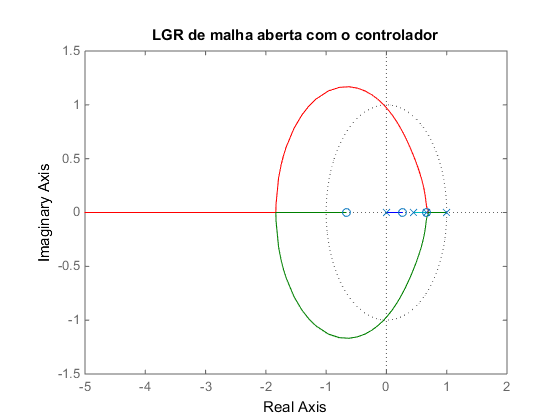
\includegraphics[width=0.8\linewidth]{Figuras/Ch12/fig2.png}}
\end{frame}

\begin{frame}{Controlador PID discreto - Exemplo \#01}
\centerline{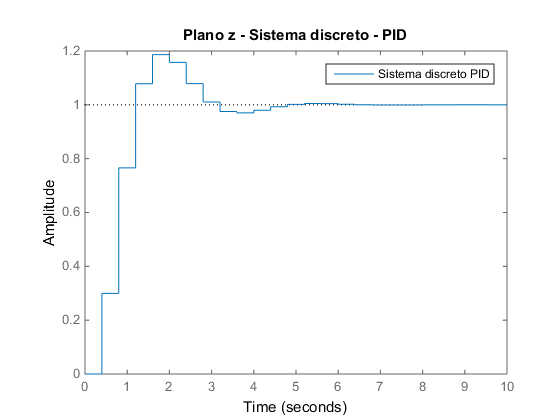
\includegraphics[width=0.8\linewidth]{Figuras/Ch12/fig3.png}}
\end{frame}

\begin{frame}{Métodos de síntese direta}
\begin{block}{Introdução}
\begin{itemize}
    \item A função de transferência em malha fechada  do sistema de controle mostrado na figura abaixo é: 
\end{itemize}
$$\dfrac{C(z)}{R(z)} = \dfrac{D(z)G(z)}{1+D(z)G(z)}$$
\end{block}
\centerline{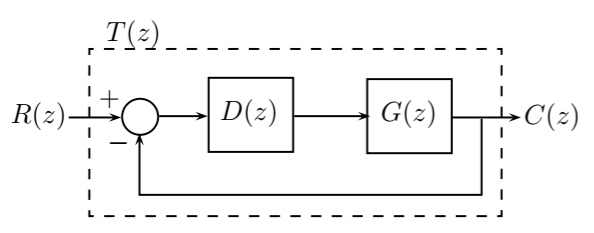
\includegraphics[width=0.8\linewidth]{Figuras/Ch12/fig4.PNG}}
\end{frame}

\begin{frame}{Métodos de síntese direta}
\begin{block}{Introdução}
\begin{itemize}
    \item Deseja-se \textbf{projetar} $D(z)$ de tal maneira  que o sistema controlado alcance certas \textbf{especificações de desempenho}. 
    \item Suponha que  tais especificações sejam atendidas por uma  função de transferência que será chamada de  \textbf{modelo de referência}: $T(z)$. 
    \item Assim, o controlador $D(z)$ deve ser tal que 
\end{itemize}
$$T(z) = \dfrac{D(z)G(z)}{1+D(z)G(z)} \implies \boxed{D(z) = \dfrac{T(z)}{G(z)[1-T(z)]}}$$
\begin{itemize}
    \item Como $D(z)$ é obtido por um cálculo direto, essa classe de técnicas é chamada de \textbf{métodos de síntese direta}. 
    \item O que diferencia os métodos dessa classe é a maneira de escolher $T(z)$. Iremos estudar dois métodos de síntese direta:
    \begin{enumerate}
        \item O controlador \textit{dead-beat};
        \item O método de Dahlin.
    \end{enumerate}
\end{itemize}
\end{block}
\end{frame}

\begin{frame}{O controlador \textit{dead-beat}}
\begin{block}{Introdução}
\begin{itemize}
    \item O controlador \textit{dead-beat} objetiva que a \textbf{resposta ao degrau} do sistema controlado seja $c(k) = 1, k = 1, 2,...$ (degrau unitário atrasado de uma unidade) nos instantes de amostragem, ou seja,
\end{itemize}
$$C(z) = \dfrac{z}{z-1} \cdot z^{-1} = \dfrac{1}{z-1}$$
\begin{itemize}
    \item Como a resposta ao degrau em malha fechada desejada é
\end{itemize}
$$C(z) = T(z) R(z)$$
\vspace{-0.3cm}
\begin{itemize}
    \item[] temos que
\end{itemize}
$$\dfrac{1}{z-1} = T(z) \dfrac{z}{z-1} \implies T(z) = z^{-1}$$
\end{block}
\end{frame}

\begin{frame}{O controlador \textit{dead-beat}}
\begin{block}{Formulação matemática}
\begin{itemize}
    \item Desta forma, o controlador \textit{dead-beat} é dado por:
\end{itemize}
$$D(z) = \dfrac{T(z)}{G(z)[1-T(z)]} = \dfrac{z^{-1}}{G(z)[1-z^{-1}]} = \dfrac{1}{G(z)[z-1]}$$
\begin{itemize}
    \item o controlador $D(z)$ determinado cancela a dinâmica da planta e \textbf{impõe a dinâmica desejada}.
    \item Em outras palavras, o numerador de $D(z)$ é composto pelo denominador de $G(z)$, ou seja, o numerador do controlador procura ``cancelar os polos da planta''.
\end{itemize}
\end{block}
\end{frame}

\begin{frame}{O controlador \textit{dead-beat} - Exemplo \#01}
\begin{block}{Problema}
	Projetar um controlador \textit{dead-beat} $ D(z) $ para 
	$$ G(s)=\dfrac{1}{(s+1)(s+2)} $$
	Considere $T=1$ s.
\end{block}
\end{frame}

\begin{frame}{O controlador \textit{dead-beat} - Exemplo \#01}
\begin{block}{Resolução}
\begin{itemize}
    \item A \textbf{discretização da planta via ZOH} (\textit{a cargo do leitor}) é:
\end{itemize}
$$G(z)=(1-z^{-1})\mathcal{Z}\left\lbrace \mathcal{L}^{-1}\eval{\left\lbrace \dfrac{G(s)}{s}\right\rbrace}_{t=kT} \right\rbrace =\dfrac{\num{0,0484}(z+\num{0,9667})}{(z-1)(z-\num{0,9048})}$$
\begin{itemize}
    \item Desta forma, o controlador \textit{dead-beat} é projetado como sendo
\end{itemize}
$$D(z) = \dfrac{1}{G(z)[z-1]} = \dfrac{(z-1)(z-\num{0,9048})}{\num{0,0484}(z+\num{0,9667})} \dfrac{1}{(z-1)} = \dfrac{\num{20,661}(z-\num{0,9048})}{z+\num{0,9667}}$$
\end{block}
\end{frame}

\begin{frame}{O controlador \textit{dead-beat} - Exemplo \#01}
\centerline{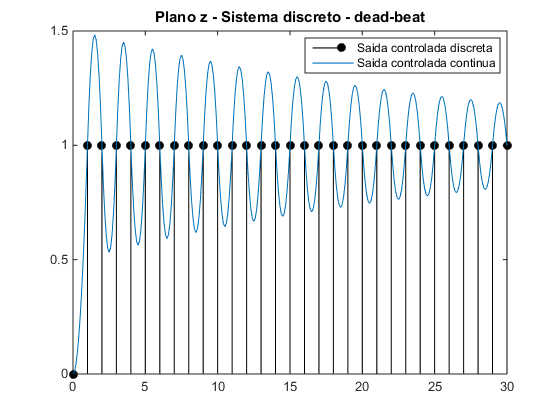
\includegraphics[width=0.8\linewidth]{Figuras/Ch12/fig5.png}}
\end{frame}

\begin{frame}{O controlador \textit{dead-beat} - Exemplo \#01}
\begin{block}{Considerações}
\begin{itemize}
    \item A saída da planta $c(t)$ \textbf{oscila} vigorosamente entre os instantes de amostragem.
    \item Além disso, a ação de controle é fortemente chaveada e requer \textbf{valores elevados}. Isso é a consequência de um \textbf{modelo de referência muito exigente}.
    \item Do ponto de vista matemático, o controlador $D(z)$ tem um polo em $z = -\num{0,9667}$, responsável pelo forte chaveamento. Tal polo é conhecido como \textit{ringing pole}. 
\end{itemize}
\end{block}
\end{frame}

\begin{frame}{O controlador \textit{dead-beat} - Exemplo \#01}
\centerline{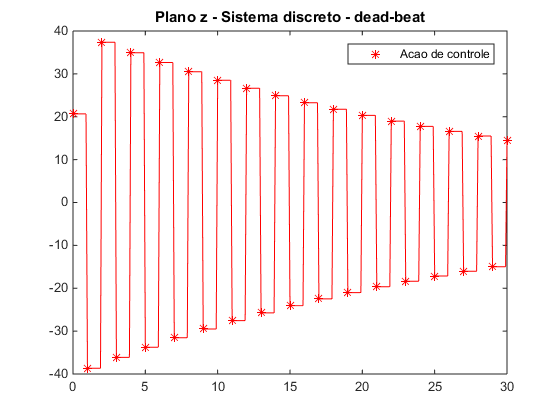
\includegraphics[width=0.8\linewidth]{Figuras/Ch12/fig6.png}}
\end{frame}

\begin{frame}{O método de Dahlin}
\begin{block}{Introdução}
\begin{itemize}
    \item Se especificarmos um $T(z)$ \textbf{menos exigente}, conseguiremos ações  de controle menos severas e a saída da planta será menos oscilatória.
    \item Deseja-se que a resposta ao degrau unitário do sistema controlado seja:
\end{itemize}
$$C(s) = \dfrac{\text{e}^{-\tau_d s}}{\tau_s + 1}\dfrac{1}{s}$$
\begin{itemize}
    \item A transformada $ \mathcal{Z} $ é dada por:
\end{itemize}
$$C(z) = \dfrac{(1-\text{e}^{-T/\tau})z^{1-n}}{(z-1)(z-\text{e}^{-T/\tau})}$$
\end{block}
\end{frame}

\begin{frame}{O método de Dahlin}
\begin{block}{Formulação matemática}
\begin{itemize}
    \item Como a resposta ao degrau em malha fechada desejada é
\end{itemize}
$$C(z) = T(z) R(z)$$,
\vspace{-0.3cm}
\begin{itemize}
    \item[] temos que
\end{itemize}
$$\dfrac{(1-\text{e}^{-T/\tau})z^{1-n}}{(z-1)(z-\text{e}^{-T/\tau})} = T(z) \dfrac{z}{z-1} \implies T(z) = \dfrac{(1-\text{e}^{-T/\tau})z^{-n}}{(z-\text{e}^{-T/\tau})}$$
\begin{itemize}
    \item Desta forma, o controlador pelo método de Dahlin é dado por:
\end{itemize}
$$D(z) = \dfrac{T(z)}{G(z)[1-T(z)]} = \dfrac{1}{G(z)} \dfrac{(1-\text{e}^{-T/\tau})}{z^{n+1}-\text{e}^{-T/\tau}z^n - (1-\text{e}^{-T/\tau})}$$
\begin{itemize}
    \item[] onde $\tau$ e $n$ são parâmetros de sintonia que  devem ser escolhidos pelo projetista. O valor de $n$ nunca deve ser menor que o atraso da planta, caso haja. 
\end{itemize}
\end{block}
\end{frame}

\begin{frame}{O método de Dahlin}
\begin{block}{Considerações}
\begin{itemize}
    \item É interessante notar que o controlador de Dahlin tem um polo em $z = 1$ para $n = 0$  e $n = 1$.
    \item Os principais comentários feitos sobre o controlador \textit{dead-beat} continuam válidos para o controlador de Dahlin. 
    \item Este, à semelhança daquele, também é baseado no  cancelamento da dinâmica da planta, o que requer um bom modelo $G(z)$.
    \item A \textbf{vantagem} do método de Dahlin comparado ao de \textit{dead-beat} é que o mesmo pode relaxar as exigências sobre o controlador, por meio da escolha de $\tau$.
\end{itemize}
\end{block}
\end{frame}

\begin{frame}{O método de Dahlin - Exemplo \#01}
\begin{block}{Problema}
	Projetar um controlador de Dahlin $ D(z) $ para $$ G(s)=\dfrac{1}{(s+1)(s+2)} $$
	Considere $T=1$ s.
\end{block}
\end{frame}

\begin{frame}{O método de Dahlin - Exemplo \#01}
\begin{block}{Resolução}
\begin{itemize}
    \item Como ponto de partida, considere $n=0$ e $\tau = 5$ s.
    \item A \textbf{discretização da planta via ZOH} (\textit{igual ao exemplo anterior}) é:
\end{itemize}
$$G(z)=(1-z^{-1})\mathcal{Z}\left\lbrace \mathcal{L}^{-1}\eval{\left\lbrace \dfrac{G(s)}{s}\right\rbrace}_{t=kT} \right\rbrace =\dfrac{\num{0,0484}(z+\num{0,9667})}{(z-1)(z-\num{0,9048})}$$
\begin{itemize}
    \item Desta forma, o controlador de Dahlin é projetado como sendo
\end{itemize}
$$D(z) = \dfrac{1}{G(z)} \dfrac{(1-\text{e}^{-T/\tau})}{z^{n+1}-\text{e}^{-T/\tau}z^n - (1-\text{e}^{-T/\tau})} = \dfrac{\num{3,7452}(z-\num{0,9048})}{z+\num{0,9667}}$$
\end{block}
\end{frame}

\begin{frame}{O método de Dahlin - Exemplo \#01}
\centerline{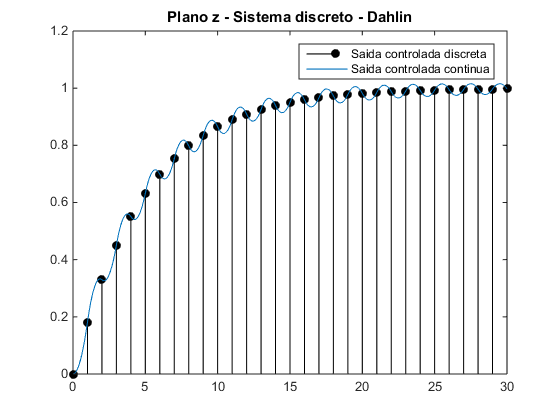
\includegraphics[width=0.8\linewidth]{Figuras/Ch12/fig7.png}}
\end{frame}

\begin{frame}{O método de Dahlin - Exemplo \#01}
\begin{block}{Considerações}
\begin{itemize}
    \item A ação de controle tem amplitude mais baixa do que no caso do controlador \textit{dead-beat}, mas ainda é bastante chaveada.
    \item Além disso, a saída da planta não difere muito da saída do modelo discreto,  ou seja, $c(t)$ não se afasta dos valores de $c(k)$ entre os instantes de amostragem.
\end{itemize}
\end{block}
\end{frame}

\begin{frame}{O método de Dahlin - Exemplo \#01}
\centerline{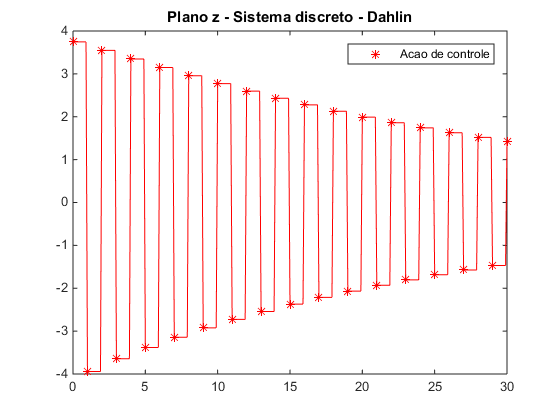
\includegraphics[width=0.8\linewidth]{Figuras/Ch12/fig8.png}}
\end{frame}

\begin{frame}{O método de Dahlin - Exemplo \#01}
\begin{block}{Resolução}
\begin{itemize}
    \item Considere agora $n=1$ e $\tau = 2$ s.
    \item A \textbf{discretização da planta via ZOH} (\textit{igual ao exemplo anterior}) é:
\end{itemize}
$$G(z)=(1-z^{-1})\mathcal{Z}\left\lbrace \mathcal{L}^{-1}\eval{\left\lbrace \dfrac{G(s)}{s}\right\rbrace}_{t=kT} \right\rbrace =\dfrac{\num{0,0484}(z+\num{0,9667})}{(z-1)(z-\num{0,9048})}$$
\begin{itemize}
    \item Desta forma, o controlador de Dahlin é projetado como sendo
\end{itemize}
$$D(z) = \dfrac{1}{G(z)} \dfrac{(1-\text{e}^{-T/\tau})}{z^{n+1}-\text{e}^{-T/\tau}z^n - (1-\text{e}^{-T/\tau})} = \dfrac{\num{8,1295}(z-\num{0,9048})}{(z+\num{0,9667})(z+\num{0,3935})}$$
\end{block}
\end{frame}

\begin{frame}{O método de Dahlin - Exemplo \#01}
\centerline{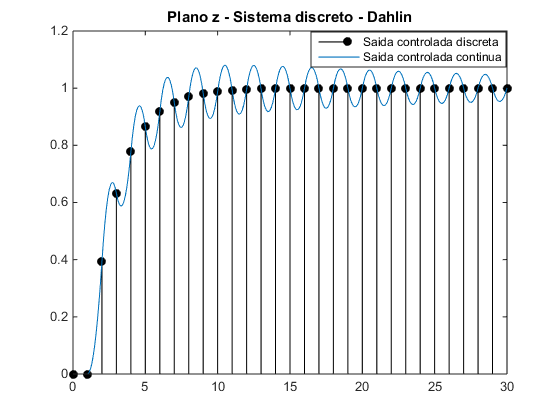
\includegraphics[width=0.8\linewidth]{Figuras/Ch12/fig9.png}}
\end{frame}

\begin{frame}{O método de Dahlin - Exemplo \#01}
\begin{block}{Considerações}
\begin{itemize}
    \item Como esperado, à medida que o modelo de referência torna-se mais exigente, a saída da  planta entre os instantes de amostragem torna-se oscilatória, além de um aumento no esforço de controle.
\end{itemize}
\end{block}
\end{frame}

\begin{frame}{O método de Dahlin - Exemplo \#01}
\centerline{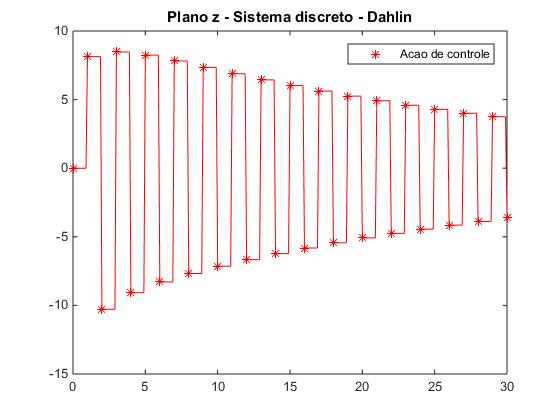
\includegraphics[width=0.8\linewidth]{Figuras/Ch12/fig10.png}}
\end{frame}


\frame{
\frametitle{Exercícios}
\begin{block}{}
01. Projete o controlador PID discreto, visto em sala de aula, por meio da imposição algébrica dos polos.

\vspace{0.7cm}

02. Raízes da equação característica que possuem partes reais próximas ao valor $-1$ (mas dentro do círculo unitário) mostram um comportamento fortemente oscilatório, denotado como \textit{ringing}. Por que? Pesquise sobre.
\end{block}
}

\frame{
\frametitle{Referências e exercícios complementares}
\begin{itemize}
\item AGUIRRE, Luis A. Controle de Sistemas Amostrados, 1 ed. [s.n.], 2019.
\end{itemize}
\centering{\alert{Página 234 - \textbf{Capítulo 6}}} \\
\vspace{0.4cm}
\begin{itemize}
\item FRANKLIN, Gene F.; POWELL, J. David; WOLKMAN, Michael L. Digital Control of Dynamic Systems, 3 ed. Addison-Wesley, 1998.
\end{itemize}
\centering{\alert{Página 270 - \textbf{Capítulo 7}}} \\
}